In the previous chapter we explored the concept of Kanji \textbf{importance}. In that point of the process, we associated the importance of a Kanji solely with its frequency in the Japanese language, in a way that more frequent Kanji are seem as more important than less frequent Kanji. In this chapter we will explore relations between Kanji to try and reach a more reasonable measure of importance.

There is in Computer Science a field of study that concerns itself with the study of mathematical structures that model pairwise relations between objects, the Graph Theory. In this chapter we will bring together our existent need to better rank the importance of Kanji with the existent solutions relative to Graph Theory.

\section{The PageRank Algorithm}
In 1998, Larry Page et al. published a paper that radically changed the scene for web search\cite{page1999pagerank}. In this paper they describe an algorithm devised to rank web pages objectively and mechanically, measuring the human interest and attention devoted to each page. In this paper they also compare the PageRank algorithm with an idealized random Web surfer, a comparison that will be useful for our application.

This algorithm estimates the rank of web pages based on the structure of hyperlinks that exist between t
hese pages. Figure \ref{fig:pagerank} shows an example graph and the solution to the ranking algorithm in this case.

\begin{figure}[ht]
    \centering
    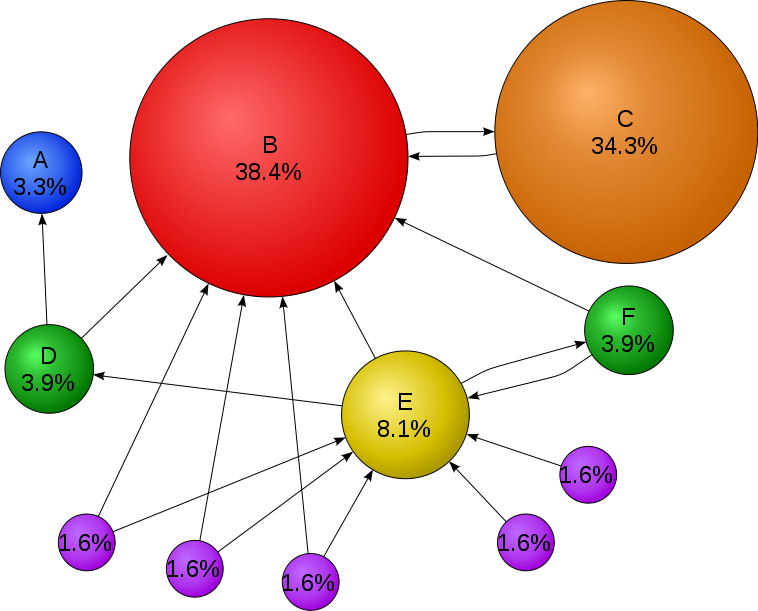
\includegraphics[width=0.75\linewidth]{Cap4/PageRankExample}
    \caption{Example of the ranking done by PageRank}
    \label{fig:pagerank}
\end{figure}

We can think of this algorithm as a flow for influence from pages, one that does not just count incoming links and outgoing links, but rather takes in consideration the influence of the page where this link is coming from, which is also calculated by this same algorithm, recursively. For example, in this graph we note that the rank for node "E" is smaller than the rank of node "C", even though the first has many more incoming links than the second. In this case, it can be seen that the pages that refer to "E" are of minor importance, while "C" is the only page hyperlinked from "B".

The second view that was described as useful for this algorithm is the random surfer abstraction. PageRank behaves as an estimate of the probability that of the node where the random surfer could be found in the graph after an arbitrary long time since the start starting from any node. His behavior would be to start at an arbitrary page on the web and than start a game of arbitrarily following hyperlinks to other pages. This representation allows us to find some problems that should be addressed at this point of the description, which are based on where the surfer can or can not go at any given point: the rank sinks.

\subsubsection{Dead Ends}
Let's firstly analyse dead ends, pages that have no outgoing link. At this point, our random surfer would get stuck in that page forever. That way, after a long enough time in the graph our imaginary surfer would get stuck in the dead end and the probability to find it there would be one (if only one such page existed). In the mathematical representation of this problem, it can be noted that the importance of the graph will "leak out" through such nodes, since those pages have no other pages to share its importance with. In the example picture, node "A" is a dead end.

\subsubsection{Spider Traps}
Spider traps are a similar kind of threat to our calculation, but it is more subtle one. Instead of being points where the user can't go anywhere else, spider traps are regions of the graph where the user would get stuck between pages from that region, with no outgoing links to other regions of the graph. One such case in the example Figure \ref{fig:pagerank} are nodes "B" and "C", that although both of them are not dead ends, once any user enters through "B" he would be stuck going back and forth between "B" and "C", and another case would happen if the "A" link had a link to itself. In these cases, all of the influence from the web would be drained by these regions.

\subsection{Random Teleports}
To solve this problem, Page et al.\cite{page1999pagerank} proposed the use of a vector parameter that would be responsible for random jumps in the graph. According to their description, the web surfer would get "bored" from time to time and jump to an arbitrary web page with probability $1-\beta$. Furthermore, in the case of dead end nodes the chance to jump to another random node would be one. 

\subsection{Non-Homogeneous Random Teleports}
Though this approach is sufficient for a basic rating of the web\footnote{Not that albeit this was the original algorithm for Google's search engine, many other papers were forwarded creating a better understanding of the topic, including an algorithm to counter-attack spam attempts: TrustRank}, it may be altered to be used for other objectives. This type of customization is commonly referred as Personalized PageRank, including by its creators\cite{page1999pagerank}. Although it is important to have random teleports to solve problems of dead ends and spider traps, there's no mathematical restriction that requires this teleport to be over \textbf{all} nodes of the graph or that this teleport should pick a jump node with equal probability for every node. The only requirement is that the jump probabilities make up for a total of 100\%.

One example of an application that personalizes the jump vector is the called Topic-Sensitive PageRank\cite{haveliwala2002topic}. This approach forces the random jump to be done to a page that is identified as being of a certain topic, so that the random restarts always come jump back not to any point of the web, but a very specific restart set. With this approach, it is possible to rank pages that are identified as being of a certain topic as well as pages that can be found after a small random walk from those pages.

This academic work focuses in another personalization of the jump vector: the non-homogeneous random teleports. In this approach, instead of giving an equal chance to all the nodes to be the targets of the random jump, we can skew the probabilities so that some nodes are more probable than others. For example, imagine a simple graph with three nodes. With homogeneous random restarts we would have a probability of $1/3$ to jumping to any node of the graph. If we use non-homogeneous random restarts however, it is possible to define a jump vector such as:
\[
\begin{bmatrix}
0.5 \\
0.3 \\
0.2
\end{bmatrix}
\]

With this application we can arbitrarily favour nodes in the graph as we see fit to the application at hand.

\subsection{Mathematical Representation}
Now that we've explained all the base intuition to the PageRank algorithm and the abstraction of the random web surfer, it is important that we also show the mathematical and computational base that can be used to implement these concepts.
\subsubsection{Flow Formulation}
Firstly, we can define mathematically the rank of a page $j$ as:
\[
r_j = \sum_{i \rightarrow j} \dfrac{r_i}{d_i}
\]
Where $j$ is a page, $i \rightarrow j$ represents all pages that point to $j$ and $d_i$ is the degree of $i$, measured as the number of outgoing links of $i$.
That is to say, the rank of a page j is the summation of the rank contributed by each of its incoming links, where each page contributes to the rank of each of its pointed pages by a fraction of its own rank and the number of pages it points. That being so, we consolidate our perspective that pages that point to many other pages will spread their influence among these, while pages that point to just a few will concentrate its influence on those. Note that since we start the process without knowing any of the ranks of the nodes, we end up with a system of $N$ variables and $N$ equations. To better solve this problem, we can condense all those equations in a matrix.

\subsubsection{Matrix Formulation}
The matrix that can be created to represent the mentioned flow equations is called an stochastic adjacency matrix. It is named as so because each column sums to 1 (since the outgoing link is spread evenly between its outgoing links). To illustrate this process and the resulting links, we introduce an example graph to be solved, which is presented in Figure \ref{fig:graphexample}.

\begin{figure}[ht]
    \centering
    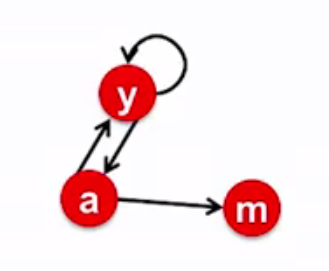
\includegraphics[width=0.4\linewidth]{Cap4/SmallGraph}
    \caption{An example of a small graph}
    \label{fig:graphexample}
\end{figure}

In this graph, we can write the flow equations as:
\begin{align*}
r_y &= \dfrac{1}{2}r_y + \dfrac{1}{2}r_a \\
r_a &= \dfrac{1}{2}r_y \\
r_m &= \dfrac{1}{2}r_a
\end{align*}
Note that at this point $r_m$ only appears once, since it is a dead end.

To turn this into a matrix we can write:
\[
\begin{bmatrix}
r_y \\
r_a \\
r_m
\end{bmatrix}
=
\begin{bmatrix}
1/2 & 1/2 & 0 \\
1/2 & 0 & 0 \\
0 & 1/2 & 0
\end{bmatrix}
\begin{bmatrix}
r_y \\
r_a \\
r_m
\end{bmatrix}
\]
That is, given that page $i$ has $d_i$ out-links, we set $M_ji=\dfrac{1}{d_i}$ if page $i$ points to page j, otherwise $M_ji=0$.

\subsubsection{Teleport Vector}
The matrix we've seen so far is similar to the Markov transition matrix. We can benefit from this proximity to use a result known for Markov chains:
\begin{center}
\textit
For any start vector, the power method applied to a Markov transition matrix \textbf{P} will converge to a unique positive stationary vector as long as \textbf{P} is stochastic, irreducible and aperiodic.\cite{pakes1969markov}
\end{center}
So, as discussed earlier, our transitions matrix can be made stochastic, irreducible and aperiodic by adding a stochastic column vector to all columns of this matrix\footnote{It is important to note that this can be any stochastic vector as long as all elements are different than zero. If some elements are equal to zero, we can not guarantee that the final matrix has these properties.}. Also, it is important that all columns that sum to zero (dead-ends) have 100\% probability to jump to a node from the restart set. If we use the homogeneous case we can do a pre-processing step to fix the $A$ matrix as:
\[
\begin{bmatrix}
1/2 & 1/2 & 0 \\
1/2 & 0 & 0 \\
0 & 1/2 & 0
\end{bmatrix}
\rightarrow
\begin{bmatrix}
1/2 & 1/2 & 1/3 \\
1/2 & 0 & 1/3 \\
0 & 1/2 & 1/3
\end{bmatrix}
\]
And also rewrite our base equation as:
\[
\begin{bmatrix}
r_y \\
r_a \\
r_m
\end{bmatrix}
=
\Bigg(
\beta \cdot
\begin{bmatrix}
1/2 & 1/2 & 1/3 \\
1/2 & 0 & 1/3 \\
0 & 1/2 & 1/3
\end{bmatrix}
+
(1-\beta) \cdot
\begin{bmatrix}
1/3 & 1/3 & 1/3 \\
1/3 & 1/3 & 1/3 \\
1/3 & 1/3 & 1/3
\end{bmatrix}
\Bigg)
\begin{bmatrix}
r_y \\
r_a \\
r_m
\end{bmatrix}
\]
If we now name the rank vector as $r$, our stochastic adjacency matrix as $M$ and the teleport matrix as $H$ we can rewrite the equation as:
\[
r = (\beta \cdot M + (1-\beta) \cdot H) \cdot r
\]
And we can proceed in naming $A = \beta \cdot M + (1-\beta) \cdot H$ to yield our final equation:
$$r = A \cdot r$$

\subsubsection{Solution Through Eigenvector calculation}
If we closely inspect the final equation for the PageRank calculation, we note that our equation in in the form
$$\lambda x = A \cdot x$$
that is, our equation represents the calculation of the eigenvector correspondent to the eigenvalue where $\lambda = 1$.

Since each column of $M$ sums to one and $r$ is a stochastic vector, we have that $Mr \leq 1$, so the sought after eigenvector is in fact the first or principal eigenvector. 

\subsubsection{Solution Through Power Iteration}
Although we could use a linear algebra package to solve our final equation, we have in hands a more efficient method to calculate a single eigenvector which has its eigenvalue known: the power iteration method. With this method, we start initializing $r^{(0)} = [1/N,...,1/N]^T$, and we iterate $r^{(t+1)} = M \cdot r^{(t)}$ as long as $|r^{(t+1)} - r^{(t)}|_1 > \epsilon$, where $|x|_1$ represents the $L_1$ norm of $x$\cite{arasu2002pagerank}.

Although other approaches designed to work at the scale of million of nodes exist, this method is efficient enough for the calculation of a problem as small as the determination of ranks of the 2,136 Jouyou Kanji.

\section{Modeling the study of Japanese Kanji as a PageRank Problem}
Well, now we know what to do, let's fetch some matrices!
\subsection{The Morphological Graph}
It exists cause they look like, are contained and contain each other.
Some examples.
\subsubsection{Creating the Morphological Graph}
By hand. Tragic.
Don't forget to speak about the frigging squares.
\subsubsection{Creation of the Relationships Matrix}
\subsubsection{Refining result to remove misc characters}
It is not just Jouyou Kanji that can be part of other Jouyou Kanji. Radicals, uncommons, Chinese only...

\subsection{The Co-occurrence Graph}
Words exist.
\subsection{Creating the Co-occurrence Graph}
\subsubsection{Creation of the Relationships Matrix}
\subsubsection{Managing occurrences with misc characters}

\section{Results}